\documentclass[12pt,letterpaper]{article}

%% Artificial Life (MIT Press) journal initial-submission format: SINGLE-COLUMN, DOUBLE-SPACED, APA-style
%% (was the ALIFE conference 2-column class `alifeconf`, reused from the LBA only to bootstrap a PDF).
\usepackage[T1]{fontenc}  %% scalable Type 1 encoding (avoid Type 3 bitmap fallback under pdflatex)
\usepackage{lmodern}      %% Latin Modern: scalable body font, no Type 3
\usepackage{natbib}
\usepackage[margin=1in]{geometry}
\usepackage{graphicx}  %% was provided by alifeconf; needed for \includegraphics
\usepackage{setspace}
\usepackage{microtype}  %% reduce overfull hboxes
\doublespacing
\emergencystretch=3em
\sloppy
\usepackage{amsmath}
\usepackage{url,hyperref,cleveref}
\hypersetup{hidelinks,
  pdftitle={A Decodable Signalling Code Co-evolves but Stays Private to Kin: Survival Selection, Clonal Descent, and Why No Public Code Bootstrapped in a Minimal World},
  pdfauthor={Chunxuan Yang}}
\usepackage{booktabs}
\usepackage{placeins}

\newcommand\blfootnote[1]{%
  \begingroup
  \renewcommand\thefootnote{}\footnote{#1}%
  \addtocounter{footnote}{-1}%
  \endgroup
}

\title{A Decodable Signalling Code Co-evolves but Stays Private to Kin:\\
Survival Selection, Clonal Descent, and Why No Public Code\\
Bootstrapped in a Minimal World}

\author{
    Chunxuan Yang \\
    \mbox{}\\
    Sogang University, Seoul, Republic of Korea \\
    yang2023@sogang.ac.kr \quad yangchunxuan1@gmail.com
}

\begin{document}
\maketitle

\begin{abstract}
We ask whether a decodable signalling code can \emph{grow} from random weights under
survival selection alone (no gradient on the task, no oracle labels, no borrowed
weights), and whether what grows is a public shared convention or a private kin code.
In a minimal hand-coded 2-D lethal-vent world, tiny tied code-table agents evolve a
decodable communication channel, and we decompose the result. Both arms carry the full
code-table; the only manipulated variable is the reproduction-fitness signal (survival
vs.\ uniform-random, with the reproduction RNG byte-matched between arms). The
tied-architecture-plus-clonal-descent baseline alone (the random-fitness control, which
also fixates to \textasciitilde{}one lineage) reaches mutual intelligibility (MII) 0.1174,
already \textasciitilde{}73$\times$ the 1/625 $\approx$ 0.0016 chance floor; at the
pre-registered gen-28 fixation point survival selection adds a paired win-margin of
\textbf{+0.0548} on top (95\% CI [0.0234, 0.0849], $n{=}48$; survival arm MII 0.17219
vs.\ random-fitness control 0.1174). Selection therefore \emph{sharpens and tunes} a
largely descent-determined channel rather than originating it from nothing. A secondary,
post-hoc transient probe ($n{=}24$, checkpoints at gen 28/56/100/150) shows this margin
is a \textbf{transient acceleration}, not a sustained equilibrium difference: the
survival-arm MII stays \textasciitilde{}stable (\textasciitilde{}0.16--0.17) while the
random-fitness control's MII rises (0.117 $\to$ 0.138) as clonal fixation alone
accumulates cross-agent decodability, so the paired margin decays from
+0.0569 [0.0162, 0.1021] (gen 28) through +0.0489 [0.0151, 0.0821] (gen 56)
to +0.0329 [$-$0.0014, 0.0687] (gen 100) and +0.0249 [$-$0.0072, 0.0571] (gen 150).
Within-kin decodability is thus fundamentally a clonal-descent phenomenon that survival
selection merely \emph{accelerates}. The code stays private to \emph{kin}: the survival
arm fixates to a single founder lineage (mean dominant-lineage share 99.1\%, N$_{\rm eff}$ 1.02),
so within-founder intelligibility runs \textasciitilde{}0.16 (\textasciitilde{}100$\times$
chance) while cross-founder intelligibility sits at the chance floor. Three heterogeneous
interventions that triangulate cross-lineage pressure all leave cross-founder
intelligibility at chance; under these regimes a public cross-lineage code did not
bootstrap (positive-or-inconclusive tier, not banked as a formal negative). The
co-evolution headline is scoped to this world, this architecture, and a 28-generation
timescale. Methodologically, we contribute a bidirectional self-audit whose single claim
is \textbf{bidirectionality}: it is built to catch deflation as well as inflation. In this
project it caught a pilot/formal false \emph{negative} and an RNG-offset bug in the headline
control, whose fix left the conclusion intact and slightly strengthened the margin
(+0.045 $\to$ +0.0548).
\end{abstract}

Code \& data: all source, the hand-coded world, the experiment runners, and every banked verdict JSON are openly available at \url{https://github.com/yangchunxuan/grown-grounded-language}; every result regenerates via the commands in the Appendix. An archival snapshot is deposited at Zenodo, DOI \url{https://doi.org/10.5281/zenodo.21074235} (concept DOI, always resolving to the latest version).\\
\blfootnote{\textcopyright{} 2026 Chunxuan Yang. Published under a Creative Commons Attribution 4.0 International (CC BY 4.0) license.}

\textbf{Keywords:} artificial life; emergent communication; signalling code; survival selection; clonal descent; kin selection; adversarial self-audit methodology

%% ─────────────────────────────────────────────────────────────────────────────
\section{Introduction}

Where does a shared signalling code come from? A communication channel is \emph{decodable}
when a receiver can recover a signal's referents from the signal alone, and a code is
\emph{public} when distinct lineages (not just kin) can decode one another. Most
computational accounts of how such a code arises take one of two routes. In the
signalling-game and reinforcement tradition, communication is \emph{trained in}: a channel
is optimised by gradient descent on a task with a differentiable channel
\citep{foerster2016}, or by reward on a referential task that supplies a task signal each
round \citep{lazaridou2017}. In the iterated-learning tradition, structure is \emph{induced
by design}: a transmission bottleneck is imposed between generations so that only learnable,
compressible codes survive \citep{kirby2008}. Both routes answer a real question,
but neither asks the more basic one we take up here: can a decodable signalling code
\textbf{grow} (neither designed-in nor trained-in) from random initial weights under
\textbf{survival selection alone}, with no gradient on the communicative task, no oracle or
truth labels, and no borrowed or pretrained weights? And if such a code does grow, is it a
\textbf{public} code shared across the population, or a \textbf{private} code confined to
kin?

We study this question in a deliberately minimal substrate: a hand-coded, fixed-rule 2-D
lethal-vent world in which agents metabolise, can die, and reproduce, and in which a tiny
tied code-table (the only communicative apparatus) is initialised from $\mathcal{N}(0,1)$
noise. The world is not learned and the channel is not optimised; the sole pressure on
communication is that organisms that use it must, on average, survive and reproduce more.
Mutual intelligibility (MII) is measured not by weight similarity but as inter-agent
codebook agreement: a sampled set of referents is passed through one agent's emission and
another's decoding, and we score exact-tuple recovery against a chance baseline of
$1/625 \approx 0.0016$. This minimality is the point: a small world makes the mechanism
legible and lets us build a control that is matched to the experimental arm in every respect
except the reproduction-fitness signal.

The scientific contribution is a single, scoped finding with three parts. First, within this
world and over a 28-generation timescale, a decodable channel \textbf{co-evolves from
scratch}, but the result decomposes into a descent baseline and a selection increment. The
control (the \textbf{random-fitness control}) also fixates to \textasciitilde{}one lineage,
so its MII of \textbf{0.1174} (already \textasciitilde{}73$\times$ the 1/625 chance floor)
is the tied-architecture-plus-clonal-descent baseline, not zero. At the pre-registered
gen-28 fixation point, survival selection adds \textbf{+0.0548} on top (95\% CI
[0.0234, 0.0849], $n{=}48$). A secondary post-hoc transient probe shows this gen-28 margin
is a \textbf{transient acceleration} of clonally-shared decodability rather than a sustained
equilibrium difference. Second, this code is \textbf{not public}. The survival arm fixates
to a single founder lineage (mean dominant-lineage share \textbf{99.1\%}, N$_{\rm eff}$
\textbf{1.02}), so the co-evolved code is a \textbf{kin code}. Third, actively maintaining
lineage diversity is \emph{necessary but not sufficient}. In the one sustained-diversity
cell (soft96, $n{=}8$) coexisting non-kin lineages still decode one another only at the
floor, and putting cross-lineage decoding directly under selection does not bootstrap a
public code: higher pressure only crashes survival. We name this a
\textbf{pressure-vs-survival tension}.

The second contribution is methodological: a reusable self-audit whose single
methodological claim is \textbf{bidirectionality}, that it catches \emph{deflation} as
readily as inflation. We demonstrate this with two in-scope catches reproducible from this paper's
own artifacts: a pilot/formal false \emph{negative} and an RNG-offset bug in the headline
random-fitness control (whose fix slightly strengthened the margin, +0.045 $\to$ +0.0548).

%% ─────────────────────────────────────────────────────────────────────────────
\section{Related Work}

Our study sits at the intersection of five lines of work and is shaped by a sixth:
a methodological critique about over-claimed emergence and weak baselines.

\textbf{Emergent communication in MARL.} A large body of deep multi-agent
reinforcement-learning work shows that communication protocols arise when agents are jointly
optimized on a task, typically with a differentiable or otherwise privileged channel
\citep{foerster2016}, or are scored by reward on a referential task that supplies a task
signal on every round \citep{lazaridou2017}. Grounded compositional language can emerge in
multi-agent populations under such task-optimized training \citep{mordatch2018}, and the
modern deep-emergent-communication literature is broad enough to have its own reviews and
tooling \citep{lazaridoubaroni2020,kharitonov2019}. Our setup deliberately removes these
affordances. There is no gradient on the channel and no oracle: adaptation proceeds by
mutation and selection on survival alone.

\textbf{Signaling and convention games.} The game-theoretic tradition, from Lewis's
signaling games \citep{lewis1969} to Skyrms's evolutionary treatment \citep{skyrms2010},
establishes that stable signaling conventions can emerge from local dynamics without a
designer, and that multiple incompatible conventions can be locally stable. Our notion of a
private kin code is consistent with the existence of mutually incompatible conventions. We
offer a mechanistic instance of the convention-multiplicity that signaling theory predicts,
and measure inter-agent codebook agreement directly.

\textbf{Kin selection and signalling among relatives.} Our headline outcome is a
\emph{kin}-private code, which places it squarely in the kin-selection tradition:
relatedness lowers the threshold for cooperative and communicative traits to be favoured,
and signalling among relatives can be stable where signalling among strangers is not
\citep{hamilton1964}. In our world a private code is selectively cheap precisely because
the survival population collapses to \textasciitilde{}one founder lineage.

\textbf{Iterated learning and compositionality.} A prominent account of how structured,
transmissible language arises is iterated learning, in which a \emph{transmission
bottleneck} pressures languages toward compositional, generalizable structure
\citep{kirby2008}. Neural iterated learning realizes this pressure in deep agents and can
yield compositional structure \citep{ren2020}. At the same time, emergent-language
compositionality is not automatically tied to generalization, and agent languages can be
effective without being human-like or compositional
\citep{kottur2017,chaabouni2020}. Our design takes a pointed stance: we do
\textbf{not} impose a transmission bottleneck. Rather than building in the mechanism known
to produce shareable structure, we ask whether one is \emph{needed}.

\textbf{Artificial-life and embodied evolved communication.} Within ALife, the evolution of
communication has been studied through simulated agents under selection
\citep{cangelosi2002} and through situated, grounded language-game and robotic models
\citep{steels2003,quinn2001,marocco2007}. Our work is squarely in this lineage in spirit
but is distinguished by an explicit, architecture-matched control.

\textbf{The replication-hygiene critique.} A recurring concern is that ``language emerged''
claims are often confounded by gradient or oracle leakage, lack a matched control, and rest
on underpowered single-seed runs; relatedly, emergent protocols are often degenerate or fail
without explicit pressure \citep{kottur2017,chaabouni2020}. This critique motivates our second
contribution: a reusable adversarial self-audit combining an architecture-matched control,
multi-seed bootstrap-CI win-margins, frozen pre-registration, and a no-oracle redline.

\textbf{Positioning.} The field reliably produces public, grounded, or compositional
communication, but in lanes that supply exactly what our setting withholds: gradient-MARL
with task rewards and interacting partners \citep{mordatch2018,lazaridoubaroni2020}, a
deep-learning infrastructure for emergent-language games \citep{kharitonov2019}, imposed
iterated-learning bottlenecks \citep{ren2020}, or populations of large language models that
already possess a borrowed, pre-trained language \citep{ashery2025}. The LLM line
is a contrast case only, not a mechanism we build on. Our question is therefore not whether
public communication can be engineered (it can) but the origins/sufficiency question
those lines do not address: whether a decodable, grounded signalling code can grow from
random weights under survival selection alone, with no gradient on communication, no
oracle, and no borrowed weights.

%% ─────────────────────────────────────────────────────────────────────────────
\section{World and Agents}

The substrate is deliberately minimal and entirely hand-coded. Nothing in the world or the
agent body is learned; the only adaptive object is each agent's communication code-table,
and even that adapts by mutation and selection rather than by any gradient on the survival
task.

\subsection{The RTC lethal-vent world}

The world (\texttt{rtc\_world.py}, with constants frozen in \texttt{config/prereg\_rtc.py},
\texttt{RTC\_VERSION = "RTC-MVP0-rich-world-v1"}) is a $48\times 48$ grid carrying a
4-channel scalar field. The field evolves by a fixed-rule physics: advection, diffusion,
per-step decay, and injection from a small number of point vents per channel. These rules
are simulator code, not a trained model: the world dynamics never change in response to
agent behavior.

An agent does not read the field directly. Perception passes through a no-oracle seam:
agents receive only lagged, windowed, noisy local sensor readings plus their own body state
and any decoded messages, never the ground-truth patch value, edibility, or any founder
identity used as a policy input. The input to each agent is a \emph{lagged, noisy} sensor
read, which is why we keep our claims at ``\textbf{decodable signalling code}'' rather than
``grounded'': the channel can be decoded and is behaviourally useful, but we do not assert
that its symbols track world state per se.

Survival is metabolic. Each agent carries an energy reserve and pays a fixed upkeep every
step. When it eats, the edible value of a patch is a dot product between the local 4-channel
patch values and a fixed per-agent metabolic weight vector; the same patch is nutritious to
one metabolism and useless or toxic to another. A value below the toxic floor is immediately
lethal. Death is therefore a hard, hand-coded consequence of foraging in a flowing
field---the selection pressure the rest of the study rides on.

\subsection{The agent and its code-table}

The agent body is intentionally trivial so that communication is the only thing under
evolutionary pressure. The communicating object is a single \texttt{UnifiedIO} tied
code-table of shape $K \times \text{BANDS} \times \text{VOCAB} = 4 \times 5 \times 6$,
initialized from $\mathcal{N}(0,1)$. The table is \emph{tied}: the same parameters drive
both speaking and listening, so a mutation that changes how an agent emits also changes how
it decodes. A speaker emits by taking, per channel, the $\text{argmax}$ over the VOCAB
symbols; a listener predicts by taking, per channel, the $\text{argmax}$ over the BANDS
value-bins. This coupling is load-bearing for the convergence argument: emit and predict
cannot drift apart independently (see \Cref{fig:schematic}).

We quantify communication with mutual intelligibility (MII): a set of referents is probed
through one agent's \texttt{emit} into another agent's \texttt{decode}, scoring exact
recovery of the full tuple. The referent space is the band$\times$channel product, so
chance recovery is $1/5^4 = 1/625 \approx 0.0016$. Within-founder (WF) and cross-founder
(CF) MII are read off the off-diagonal of the full population$\times$population MII matrix,
filtered by lineage.

\subsection{Reproduction, and the from-scratch invariants}

Reproduction is mutation plus selection, with no gradient on the survival task. Offspring
are produced by adding Gaussian noise to the parent's tied code-table. Selection has two
pre-registered variants used across the arc: hard top-50\% truncation, and a soft
tournament ($k{=}2$) on lineage-shared fitness for niching.

The from-scratch invariants are strict: (i) there is \emph{no gradient on the survival
task}; (ii) the \emph{only} gradient mechanism anywhere in the codebase is an optional
cultural-imitation helper, and it is \emph{unused in every load-bearing arm} reported here;
(iii) there are \emph{no borrowed or pretrained weights and no language model}.

%% ─────────────────────────────────────────────────────────────────────────────
\section{Methods: The Attack-Machine}

Every claim in this paper is the output not of a single experiment but of a procedure built
to surface our own errors before review does. We call this procedure the
\textbf{self-audit}: six interlocking disciplines. Its single methodological claim is
\textbf{bidirectionality}: a self-audit should catch \emph{deflation} as readily as
inflation.

\subsection{The mutual-intelligibility (MII) metric}

The unit of evidence is \textbf{inter-agent codebook agreement}: can one agent decode what
another emits? For an ordered pair of agents, we sample a fixed set of referents, route each
through the speaker's \texttt{emit} and the listener's \texttt{predict}, and score
\textbf{exact-tuple recovery}. With the code-table tied at $K\times\text{BANDS}\times\text{VOCAB} = 4\times5\times6$ and a referent set of 625, chance is $1/625 \approx 0.0016$.
This unforgiving, no-partial-credit operationalization means an above-chance MII reflects a
reconstructed \emph{symbol-to-referent mapping}, not two networks that happen to look alike.

We compute MII at two scopes. \textbf{Within-founder MII (WF)} pairs agents from the same
founder lineage; \textbf{cross-founder MII (CF)} pairs agents from distinct founder
lineages coexisting at the same generation. The WF/CF split is what lets us distinguish a
\emph{private kin code} (WF high, CF at chance) from a \emph{public code} (CF also above
chance).

To guard against MII being a measurement artifact, every stage runs two pre-logged sentinels.
A \textbf{lineage-shuffle} control permutes lineage labels: if the metric truly keys on
lineage, CF should spike under shuffling---it does (CF 0.0009 $\to$ 0.065 in the
diagnostic; 15--23$\times$ across C1 cells). A \textbf{gate-0 content test} compares open
messaging against muted and scrambled channels: open $\gg$ mute/scramble with CIs excluding
zero, establishing that message \emph{content} is load-bearing.

\subsection{The architecture-matched random-fitness control}

Our control is \textbf{not} communication-ablated: \textbf{both arms carry the full
\texttt{UnifiedIO} code-table}, the same initialization, and the identical evolutionary
loop. The \textbf{only} manipulated variable is the \textbf{reproduction-fitness
signal} (survival in the treatment arm versus uniform-random in the control), with the
reproduction RNG \textbf{byte-matched between arms}. We therefore call it the
\textbf{random-fitness control}.

Crucially, this control isolates \emph{selection for communication} from \textbf{clonal
descent-convergence}: the random-fitness arm \textbf{also} fixates to \textasciitilde{}one
lineage, so its MII of \textbf{0.1174} is the tied-architecture-plus-clonal-descent
baseline (\textasciitilde{}73$\times$ the floor), not zero. At gen 28 the survival arm
reaches MII \textbf{0.17219}, a \textbf{paired} win-margin of
\textbf{+0.0548, 95\% CI [0.0234, 0.0849]}, at $n{=}48$.

This control also carries the project's two hardest lessons, both caught by the self-audit
(\S\ref{sec:method_demo}). First, a \emph{formal} treatment was once compared against a
\emph{pilot} control, manufacturing a false \textbf{negative}. Second, a multi-model
adversarial review found that an earlier version drew its fake fitness from the \emph{shared}
reproduction RNG; fixing it and re-running at $n{=}48$ left the conclusion intact and
slightly \emph{strengthened} the margin (+0.045 $\to$ +0.0548).

\subsection{Multi-seed bootstrap-CI win-margins}

We report no single-seed positives. Every load-bearing comparison runs $\geq 6$ seeds (the
headline uses 48), and the quantity reported is a \textbf{win-margin with a bootstrap
confidence interval over per-seed paired differences}. A claim counts as supported only
when the paired margin's CI excludes zero in the predicted direction. The headline check is
the random-fitness control: the survival arm beats it by the paired win-margin
\textbf{+0.0548, 95\% CI [0.0234, 0.0849]} at $n{=}48$ (\S\ref{sec:results_coevolution}).

\textbf{Multiple comparisons.} Each stage has a single, pre-registered \textbf{primary
endpoint} locked before the run. The sentinel checks (lineage-shuffle, gate-0 content,
founder-quality control) are \textbf{secondary corroborating diagnostics}, not independent
tests of the headline. We apply \textbf{no family-wise correction} by design: there is a
single locked primary per stage. The ``pressure sweep'' of \S\ref{sec:results_wall} is a
\emph{post-hoc synthesis} of three separately pre-registered probes; we treat it as
triangulation, not as a corrected family.

\subsection{Frozen pre-registration}

Each stage's specification---hypotheses, coexistence gates, outcome labels, and sample
size---is \textbf{locked in a versioned spec before the run}. Gates and labels are not moved
after seeing data. The discipline's value is most visible when it costs us something: the
diagnostic's frozen gate was met by only 5/16 seeds, forcing the pre-registered verdict
\texttt{INCONCLUSIVE\_NO\_WINDOW} even though the \emph{direction} (private codes) was
unanimous and strong.

\subsection{The no-oracle redline}

The central failure mode in this literature is leakage: an agent that secretly reads world
truth can fake communication. We draw a hard \textbf{no-oracle redline}: agent decisions
may read \textbf{only decoded messages, own body state, and legal sensors}, \emph{never}
true world patch, edibility, target-code, or founder-id-as-policy-input. A static-analysis
scan enforces a subset on the core runner.

\subsection{Code-grounded adversarial multi-agent review}

Before any spec is locked, it is attacked by independent reviewers reading the \emph{actual
runner code}, not a prose summary. This caught, e.g., the C2X ``content-free'' auto-label
as a viability-crash mislabel, and forced two reviewer contradictions in C1 to be
adjudicated on the record before locking.

\subsection{The tier rule and the provenance triple}

The \textbf{tier rule} (frozen): a run at $n \leq 8$ may only conclude POSITIVE or
INCONCLUSIVE, never a scoped negative; a negative is banked only at $n = 16$. Accordingly,
the cross-lineage CF-at-floor result is reported as ``a public code did not bootstrap under
the regimes tested'' \emph{with a stated mechanism, across seeds and across three
heterogeneous interventions}, but explicitly \textbf{not as a formal negative}.

Every result self-describes via a \textbf{provenance triple}: the immutable verdict JSON at
a git commit, the CLAIM\_LEDGER mapping each claim to its verdict-file and commit, and the
RUNBOOK giving the exact regeneration command per stage.

%% ─────────────────────────────────────────────────────────────────────────────
\section{Results}

\subsection{Co-evolution is real, but kin-scoped}
\label{sec:results_coevolution}

\begin{figure}[t]
  \centering
  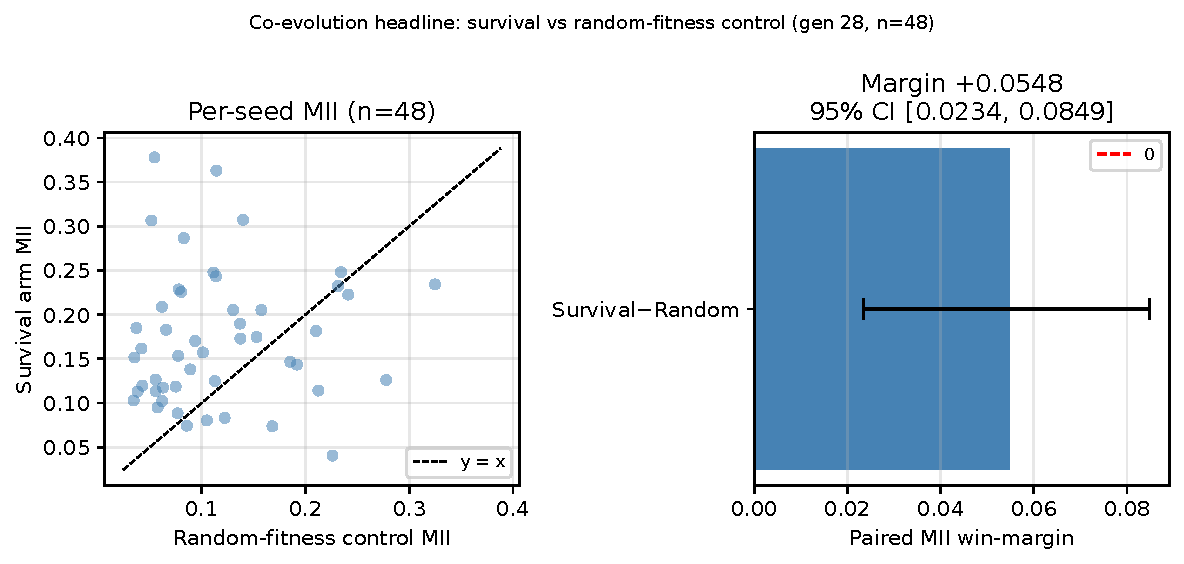
\includegraphics[width=\columnwidth]{figs/f_headline.pdf}
  \caption{Co-evolution headline ($n{=}48$, gen 28). \textbf{Left:} per-seed MII scatter:
  survival arm vs.\ random-fitness control; points above the diagonal indicate a per-seed
  win. \textbf{Right:} paired win-margin $+0.0548$ (95\% CI [0.0234, 0.0849]), CI excludes
  zero. Source: \texttt{rtc\_g1f\_commblind\_verdict\_formal48\_rngfix.json}.}
  \label{fig:headline}
\end{figure}

\begin{figure}[t]
  \centering
  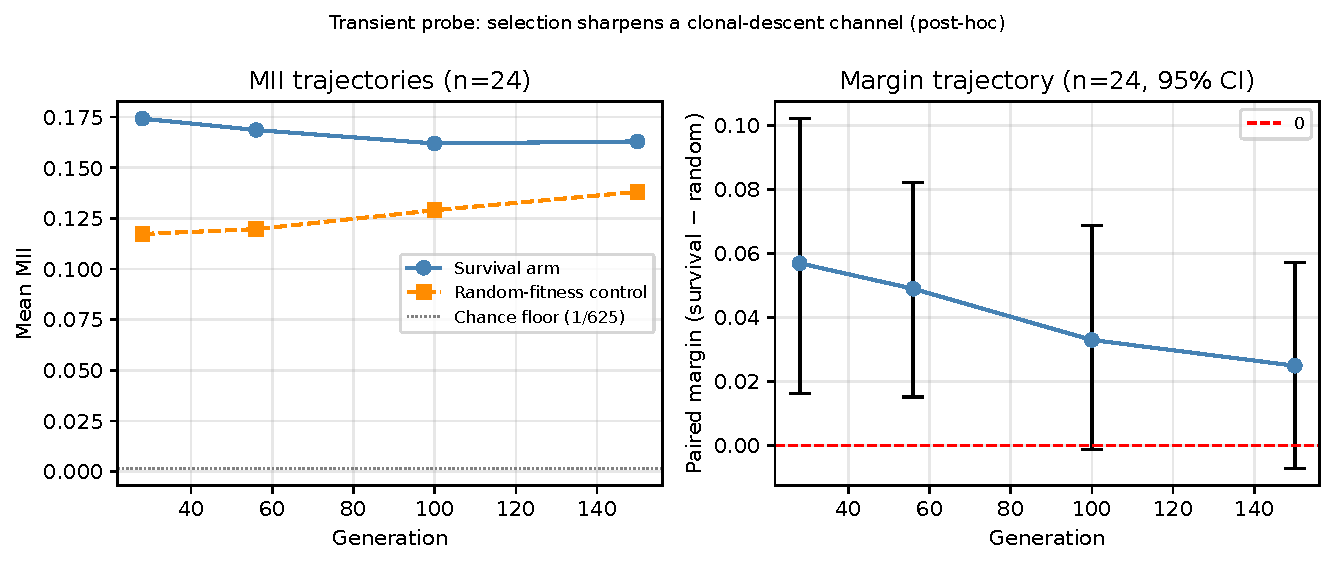
\includegraphics[width=\columnwidth]{figs/f_transient.pdf}
  \caption{Transient probe ($n{=}24$, post-hoc). \textbf{Left:} MII trajectories of both
  arms across generations 28/56/100/150. The random-fitness control rises as clonal fixation
  accumulates. \textbf{Right:} paired margin with 95\% CI decays monotonically; CI excludes
  zero at gens 28 and 56, includes zero at gens 100 and 150. Source:
  \texttt{rtc\_g1f\_transient\_probe\_verdict.json}.}
  \label{fig:transient}
\end{figure}

The first question is the existence question: does a decodable communication channel
co-evolve from random weights under survival selection alone? In the g1f configuration of
the lethal-vent world, the answer is yes, but the scope of that ``yes'' is the load-bearing
part of the result.

\textbf{The headline (a decomposition).} Under formal settings, the co-evolved channel
reaches a mean cross-agent MII of \textbf{0.17219}, against the random-fitness control at
\textbf{0.1174}. This isolates \emph{selection for communication} from
\textbf{clonal descent-convergence}: the random-fitness arm also fixates to
\textasciitilde{}one founder lineage, so its MII is not zero but the descent/architecture
baseline that any heritable code-table reaches. That baseline is already
\textbf{0.1174, \textasciitilde{}73$\times$ the 1/625 chance floor}. At the pre-registered
gen-28 fixation point, survival selection then adds a \textbf{paired} bootstrap win-margin
of \textbf{+0.0548, 95\% CI [0.0234, 0.0849]} ($n{=}48$; see \Cref{fig:headline}). The
reading is therefore a decomposition rather than an origination: the tied architecture plus
clonal descent reaches MII 0.1174 on its own, and survival selection \textbf{sharpens and
tunes} that channel by +0.0548.

\textbf{Robustness: the margin is a transient acceleration (secondary, post-hoc).} The
+0.0548 is the \textbf{pre-registered gen-28 primary} endpoint and it stands at that
timescale. A secondary, post-hoc transient probe ($n{=}24$, checkpoints at gen
28/56/100/150) shows the paired margin \textbf{decays monotonically}: gen 28
margin $+0.0569$, CI [0.0162, 0.1021] (excludes 0); gen 56 $+0.0489$, CI [0.0151, 0.0821]
(excludes 0); gen 100 $+0.0329$, CI [$-$0.0014, 0.0687] (includes 0); gen 150 $+0.0249$,
CI [$-$0.0072, 0.0571] (includes 0). The mechanism is visible in the two arms separately
(see \Cref{fig:transient}): the survival-arm MII stays roughly stable
(\textasciitilde{}0.16--0.17) while the \textbf{random-fitness control's MII rises}
(0.117 $\to$ 0.138) as single-lineage clonal fixation alone keeps accumulating cross-agent
decodability. The reading is therefore that survival selection produces a \textbf{transient
acceleration} of clonally-shared decodability rather than a sustained equilibrium
difference, and this is the empirical justification for scoping the headline to 28
generations.

\textbf{The scope (load-bearing).} The survival arm fixates to a single founder lineage:
across $n{=}48$ seeds the mean dominant-lineage share is \textbf{99.1\%} (95\% CI
[97.3\%, 100\%]), the inverse-Simpson effective number of lineages
\textbf{N$_{\rm eff} = 1.02$}, and \textbf{47 of 48} seeds end essentially single-lineage.
The co-evolved channel is therefore \textbf{kin-lineage decodability, a private kin code,
not a public cross-lineage shared convention}.

\subsection{Why kin-only? (diagnostic)}

\begin{figure}[t]
  \centering
  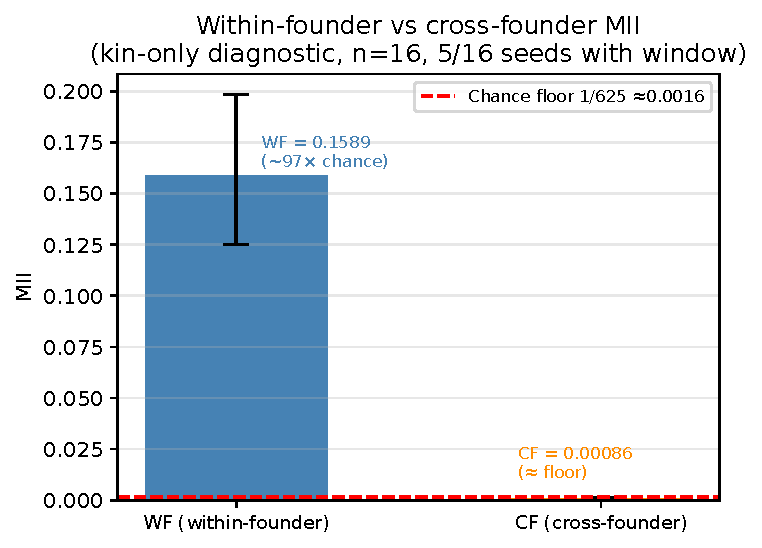
\includegraphics[width=0.7\columnwidth]{figs/f_wf_cf.pdf}
  \caption{Within-founder (WF) vs.\ cross-founder (CF) MII with chance floor (kin-only
  diagnostic, $n{=}16$, 5/16 seeds with coexistence window). WF
  $\approx 0.159$ ($\approx 100\times$ chance); CF $\approx 0.00086$ ($\approx$ floor).
  Source: \texttt{rtc\_g1f\_kinonly\_diagnostic\_verdict.json}.}
  \label{fig:wf_cf}
\end{figure}

To distinguish whether the kin-only signature is an artifact of fast founder collapse
(hypothesis A: collapse-limited) or genuine private-code divergence (hypothesis C: private
codes), we pre-registered a comparison under a frozen gate.

The frozen verdict is \textbf{\texttt{INCONCLUSIVE\_NO\_WINDOW}}: only \textbf{5/16} seeds
opened a coexistence window. We report this as inconclusive rather than relabeling the gate
after seeing the data.

The \textbf{direction}, however, is strong and unanimous, pointing to \textbf{C} (see
\Cref{fig:wf_cf}). Across the measurable seeds, within-founder MII is \textbf{0.159}
($\approx 100\times$ chance) while cross-founder MII is \textbf{0.00086} ($\approx$
chance); the ratio CF/WF is \textbf{0.5\%}, and all \textbf{5/5} measurable seeds take the
same form: whenever two non-kin lineages coexisted, they decoded each other essentially at
chance while each decoded its own kin $\approx 100\times$ above chance.

Two pre-registered sentinels rule out the obvious artifacts. (i) \textbf{Lineage-shuffle}:
permuting lineage labels lifts CF from 0.0009 to 0.065 (a \textasciitilde{}75$\times$
jump), confirming the metric truly keys on lineage membership. (ii) \textbf{Gate-0 (content
load-bearing)}: opening the channel yields MII 0.31 versus 0.03 when muted and 0.05 when
scrambled, with CIs excluding zero. The floor-level CF is genuine cross-lineage
unintelligibility, not an inert channel.

\subsection{Maintaining diversity is necessary but not sufficient}

\begin{figure}[t]
  \centering
  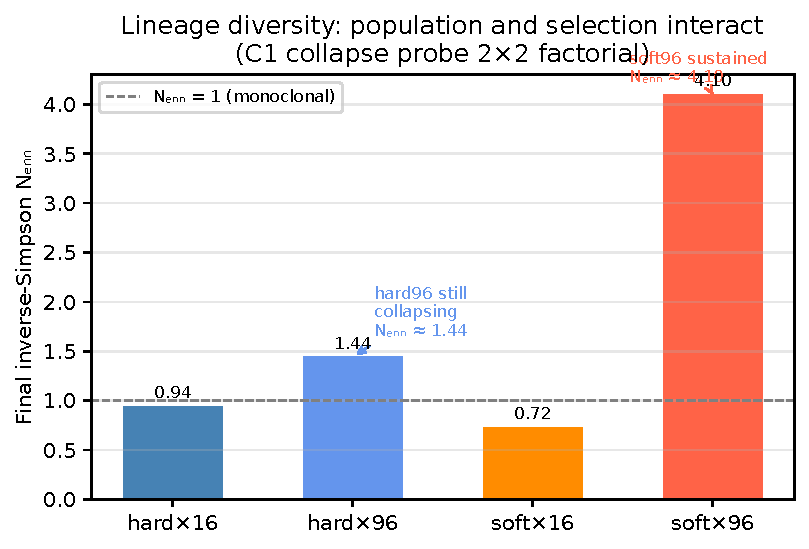
\includegraphics[width=0.75\columnwidth]{figs/f_neff.pdf}
  \caption{Final inverse-Simpson N$_{\rm eff}$ across the 2$\times$2 factorial (C1 collapse
  probe). Population size opens windows; only soft (niching) selection sustains diversity.
  Soft$\times$96: N$_{\rm eff} \approx 4.10$ (sustained); hard$\times$96:
  N$_{\rm eff} \approx 1.44$ (still collapsing). Source:
  \texttt{rtc\_g1f\_c1\_collapse\_probe\_verdict.json}.}
  \label{fig:neff}
\end{figure}

We ran a $2\times 2$ factorial---selection \{hard top-50\% truncation; soft = tournament-k2
with lineage fitness-sharing\} $\times$ population \{16, 96\}---to test whether actively
sustaining diversity lifts CF off the floor.

\begin{table}[ht]
\footnotesize
\centering
\caption{C1 collapse probe: 2$\times$2 results. WF $\approx 0.16$ across viable cells;
CF at floor ($\approx 0.0016$) throughout. All CF$-$FLOOR CIs straddle or exclude zero
from below.}
\label{tab:c1}
\begin{tabular}{@{}lrrrr@{}}
\toprule
Cell & N$_{\rm eff}$ & CF & WF & CF/WF \\
\midrule
hard$\times$16 & 0.94 (collapsed) & 0.00081 & 0.174 & 0.5\% \\
hard$\times$96 & 1.44 (collapses) & 0.00176 & 0.175 & 1.0\% \\
soft$\times$16 & 0.72 (collapsed) & 0.00072 & 0.096 & 0.8\% \\
soft$\times$96 & \textbf{4.10 (sustained)} & 0.00153 & 0.160 & 1.0\% \\
\bottomrule
\end{tabular}
\end{table}

\textbf{Mechanism: population opens windows, niching sustains them} (see \Cref{fig:neff}).
At pop=16 the population collapses regardless of selection (final N$_{\rm eff}$ 0.94 hard,
0.72 soft). At pop=96 windows open in all 8/8 seeds, but only soft selection \emph{sustains}
the diversity: hard96 still collapses to a final N$_{\rm eff}$ of 1.44, whereas soft96
ends at N$_{\rm eff}$ 4.10 in all 8 seeds, holding 15--25 coexisting generations each.

\textbf{Consistent with C, against the strong form of A (directional, $n{=}8$).} Within
soft96 (the one cell that actually delivers sustained multi-lineage coexistence),
cross-founder MII still sits at the floor: CF 0.00153 versus floor 0.0016, with the
CF$-$FLOOR confidence interval [$-$0.00031, +0.00021] straddling zero, and CF/WF $\approx 1\%$
against a within-founder MII of $\approx 0.16$ ($\approx 100\times$ chance). Preventing
collapse and sustaining 20+ generations of genuine non-kin coexistence did \textbf{not} lift
CF off the floor. Maintaining diversity is \textbf{necessary} but, on this evidence,
\textbf{not sufficient} for a shared, public code.

\subsection{The wall: no public code bootstraps}
\label{sec:results_wall}

\begin{figure}[t]
  \centering
  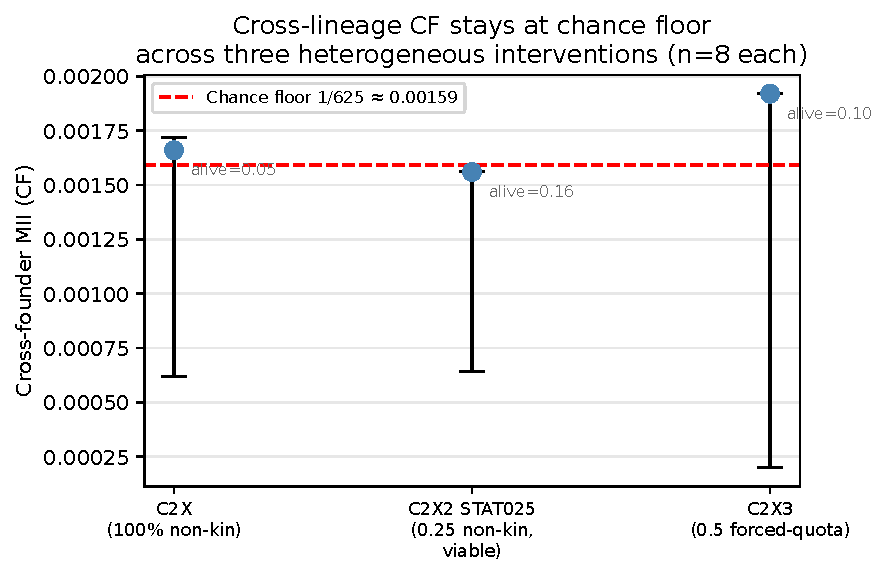
\includegraphics[width=\columnwidth]{figs/f_crosslineage.pdf}
  \caption{Cross-lineage CF stays at or below the chance floor across three heterogeneous
  interventions ($n{=}8$ each). The viable cell (C2X2 STAT025, alive $\approx 0.16$) is the
  load-bearing case; C2X crashes survival (alive 0.045); C2X3 boom-bust (alive 0.10).
  Sources: \texttt{rtc\_g1f\_c2x*\_verdict.json}.}
  \label{fig:crosslineage}
\end{figure}

Section~\ref{sec:results_coevolution} established a decodable channel that co-evolves but
stays kin-private. We then attacked the obvious rescue: if survival depends on decoding
non-kin, would a public code be selected up? We ran \textbf{three heterogeneous
interventions} (C2X, C2X2, C2X3; different designs and scaffolds, 40 vs.\ 48
generations), each locked only after code-grounded adversarial review. They are
\textbf{not} a single graded dose-response sweep; rather they \textbf{triangulate the same
null} from three directions.

\textbf{The three interventions.} The \textbf{viable cell (C2X2 stationary scaffold, 0.25
non-kin)} is the load-bearing one because the population stays alive: mean fraction alive
0.1574, clearing the pre-registered viability bar, with coexistence windows in all 8/8
seeds. Yet cross-founder MII (CF) sits at the floor: CF = 0.00156 against a chance/floor
of 0.00159, a margin of $-$0.00065, 95\% CI [$-$0.00095, $-$0.00038] (CI excludes zero), while
within-founder MII (WF) is 0.156. The \textbf{forced-quota intervention (C2X3, 0.5 non-kin)}
corroborates: mean alive 0.0998, below the viability bar, and CF never leaves the floor
(seed-aggregate CF = 0.00192, margin $-$0.00086, CI [$-$0.00139, $-$0.00032]). The
\textbf{cold 100\%-non-kin intervention (C2X)} shows the viability failure mode: mean alive
collapses to 0.0455 versus the kin-only reference of 0.2718 and the population dies before
selection can act on communication (CF\_OPEN = 0.00166, margin CI [$-$0.00097, 0.00013]
includes zero).

\textbf{Headline.} Across all three interventions, \emph{cross-founder MII never rose above
chance} (see \Cref{fig:crosslineage}). Turning the cross-lineage screw did not buy a public
code; where it bit at all, it crashed survival.

\textbf{Mechanism.} The \textbf{pressure-vs-survival tension}: non-kin codes are mutually
undecodable, so an agent forced to listen to non-kin signals receives, in effect, noise, and
acting on noise costs foraging time. A viable, diverse, \emph{converging} regime is never
reached for long enough to matter.

\textbf{Power tier.} All arms here are $n{=}8$---the POSITIVE-or-INCONCLUSIVE tier. We
therefore do not bank a FORMAL negative. We report that \textbf{a public code did not
bootstrap under the regimes tested}: CF stays at the architecture floor across all seeds
\emph{and} across all three heterogeneous interventions, with a stated mechanism. This
triangulation across heterogeneous probes is qualitatively stronger than an isolated
underpowered null. But per our calibration discipline, we claim only that under these
regimes a public code \emph{did not} bootstrap, never that this architecture \emph{cannot}
produce one.

%% ─────────────────────────────────────────────────────────────────────────────
\section{The Methodology, Demonstrated}
\label{sec:method_demo}

The preceding sections used the self-audit to defend a set of positive and null claims. This
section turns the lens around. The audit's distinctive value, its single methodological
claim, is that it runs \textbf{bidirectionally}: it is built to catch its operators
inflating a result, and it is equally built to catch them \emph{deflating} one. We anchor
this on \textbf{two in-scope, reproducible catches}: a pilot/formal false \emph{negative},
and the RNG-offset bug in the headline random-fitness control.

\textbf{It caught a false negative (\S\ref{sec:results_coevolution}).} The g1f line began
with a committed ``clean negative'': survival selection did not appear to co-evolve a
decodable channel. The self-audit exposed this as an artifact: a \emph{formal} co-evolution
arm (28 generations) had been compared against a \emph{pilot} control. The load-bearing knob
was generations (the effect plateaus around generation 12--14, and the pilot had truncated
mid-rise at 7). Re-run with both arms formal and paired at the same initialization, the
survival arm beats the random-fitness control by an MII win-margin of
\textbf{+0.0548, 95\% CI [0.0234, 0.0849]} at $n{=}48$. A real, peer-review-relevant effect
had been suppressed; the audit recovered it.

\textbf{It caught an RNG-offset bug in the headline control.} A multi-model adversarial
review found that the random-fitness control drew its fake fitness from the \emph{shared}
reproduction RNG, partially coupling the two arms. Fixing it (an independent generator for
the fake fitness) and re-running at $n{=}48$ left the conclusion intact and \textbf{slightly
strengthened} the margin, from +0.045 to \textbf{+0.0548} (survival arm 0.17219, control
0.1174, CI [0.0234, 0.0849]).

\textbf{It held a frozen gate to an honest inconclusive (\S5.2).} The kin-only diagnostic
pre-registered a coexistence gate. Only 5 of 16 seeds cleared it (founder collapse was too
fast), so the pre-registered verdict returned \texttt{INCONCLUSIVE\_NO\_WINDOW}. The frozen
gate held; we report inconclusive on the window and direction-only on the lean.

\textbf{It adjudicated two direct contradictions between independent reviewers (\S5.3).}
Locking the C1 collapse-probe spec required resolving two disagreements between independent
code-grounded reviewers (the correct fitness-sharing divisor and the coexistence-window gate
definition). The spec was locked (v5.1) only after the contradictions were explicitly
adjudicated. The machine is the forum in which reviewer disagreement is forced to a decision
before any number is generated.

\textbf{It corrected an over-coarse auto-label using a pre-logged continuous metric (\S5.4).}
The C1 window classifier emitted the binary label \texttt{POP\_DRIFT}, which undersells the
mechanism. The pre-logged continuous N$_{\rm eff}$ trajectory refined it: population size
\emph{opens} windows, but only soft/niching selection \emph{sustains} diversity. Logging a
continuous metric before knowing the answer let us correct a label that a coarse gate alone
would have shipped.

%% ─────────────────────────────────────────────────────────────────────────────
\section{Discussion}

\subsection{``Decodable but private to kin'' and what it means for language-origin theory}

The central finding of this arc is a dissociation that language-origin theory does not
usually hold apart: a communication channel can be \emph{decodable} without being
\emph{public}. Under survival selection alone, a decodable channel co-evolves from random
weights and beats an architecture-matched random-fitness control (paired win-margin +0.0548,
95\% CI [0.0234, 0.0849], $n{=}48$), with the caveat that the control already reaches 0.1174
(\textasciitilde{}73$\times$ chance) from clonal descent alone, so selection \emph{sharpens}
rather than originates the channel, and this gen-28 margin is a transient acceleration the
control's own clonal fixation closes by \textasciitilde{}gen 100. Within-founder mutual
intelligibility (WF) sits near 0.16, roughly $100\times$ the $1/625 \approx 0.0016$ chance
floor, and the content is load-bearing. Across every regime tested, cross-founder MII (CF)
never rose above chance. The code is real and it means something---but only to kin.

For theories of language origin, this matters because intelligibility is often treated as the
hard part and publicness as a near-automatic consequence. Our minimal world separates the
two. A decodable code emerged readily; publicness did not emerge at all. The reason is
mechanistic: non-kin codes are mutually undecodable, and within a single lineage there is no
selective pressure to be understood by strangers one will, in practice, almost never meet
(the formal population fixates to \textasciitilde{}99\% a single founder lineage,
N$_{\rm eff}$ 1.02). A private kin code is, in this world, an \emph{attractor}.

\textbf{What is non-obvious, relative to kin-selection and iterated-learning theory.}
\citet{hamilton1964} makes a \emph{kin-private} outcome unsurprising once relatedness is
high; iterated-learning theory predicts that \emph{shareable} structure needs a transmission
bottleneck \citep{kirby2008}. Two things in our result are not handed to us by either theory.
First, a \emph{decodable} channel emerged \textbf{without being trained or designed in}.
Second, the privacy we report is shown as ``founders never converge'': independently seeded
lineages starting at $\approx$zero cross-founder intelligibility and staying there through
20+ actively-sustained coexisting generations (C1 soft96). That a \emph{sustained-diversity}
regime still yields no convergence is the non-trivial claim.

\subsection{Why a public code plausibly needs more world, not more selection}

The natural rescue is to \emph{select for} cross-lineage understanding: make survival
depend on decoding non-kin. We did exactly this across three heterogeneous interventions. It
did not work, and the way it failed is informative. In the viable 0.25 cell the population
stayed alive (alive $\approx 0.16$) but cross-founder MII held at floor; under the 0.5
forced-quota intervention survival became boom-bust (mean alive 0.10) with CF never
exceeding 0.0058 across all seeds and generations; under cold 100\% non-kin the population
simply crashed (alive 0.045 vs.\ 0.272). Where the pressure bit at all, it only crashed
survival harder. We call this the \textbf{pressure-vs-survival tension}: forcing agents to
listen to non-kin whose codes they cannot yet decode degrades foraging and kills them before
selection can act on communication.

This points away from ``more selection pressure'' and toward ``more world.'' Two ingredients
appear to be missing: first, \textbf{shared referents worth naming}; second,
\textbf{sustainable diversity under communication pressure}. A public code presupposes
multiple lineages that both persist \emph{and} benefit from understanding one another. We
showed that maintaining diversity is necessary but not sufficient: niching (tournament
selection plus lineage fitness-sharing) sustained genuine multi-lineage coexistence at
pop=96 (soft96 final N$_{\rm eff}$ 4.10, 8/8 seeds, 15--25 coexisting generations), yet
cross-founder MII still sat at the floor.

\subsection{Relation to the iterated-learning bottleneck}

We deliberately did \emph{not} impose a transmission bottleneck \citep{kirby2008}. Our
agents inherit weights by mutation and selection, not by learning from a teacher through a
narrow channel. The pressure-vs-survival tension we observe can be read as suggesting
\emph{why} such a bottleneck, or an ecological analogue of one, may be a prerequisite for
a public code: without a mechanism that repeatedly forces codes through a shared, learnable
interface, lineages drift into mutually private dialects and there is no force pulling them
back together. We frame this as a hypothesis the arc \emph{motivates}, not a result it
establishes.

\subsection{Honest limits}

These claims are scoped narrowly and on purpose. They hold for \textbf{one hand-coded world}
(the RTC lethal-vent substrate), \textbf{one architecture} (the tied UnifiedIO code-table,
random $\mathcal{N}(0,1)$ init), and \textbf{per-stage timescales} (28 generations for the
headline co-evolution, kin-only diagnostic, and C1 arms; 40--48 generations for the
cross-lineage pressure probes). The headline co-evolution result is well powered ($n{=}48$),
though its absolute margin is modest and decomposes into a clonal-descent baseline (MII
0.1174) plus a selection increment (+0.0548) that a secondary, post-hoc transient probe
($n{=}24$) shows is a \textbf{transient acceleration} that decays to a CI including zero by
\textasciitilde{}gen 100. The cross-lineage outcome is \emph{not} a formal negative: a public
code ``did not bootstrap under the regimes tested ($n{=}8$, positive-or-inconclusive tier),
across three heterogeneous interventions, with a stated mechanism.'' We make no impossibility
claim.

\textbf{Why 28 generations suffices for the bootstrap question.} A reviewer may reasonably
ask whether running pop=96 for thousands of generations would let mutation eventually break
the kin-private wall. We argue it would not. First, bootstrapping a public code is an
\emph{initiation} question, not an \emph{equilibrium} one: a public code that was going to
emerge would first show cross-founder MII lifting off the floor during sustained coexistence
and then amplifying. In the soft96 cell we sustained 20+ generations of genuine multi-lineage
coexistence (N$_{\rm eff}$ 4.10) and CF never lifted even partially, so there is no nascent
signal for additional generations to amplify. Second, no mechanism supplies a force toward
cross-lineage alignment: independently seeded code-tables occupy a 625-referent space in which
mutual intelligibility by drift alone is a near-measure-zero coincidence
(chance $\approx 1/625$ per referent), and selection actively \emph{opposes} alignment through
the pressure-vs-survival tension. Additional generations add drift, not a new directional
force. Third, the regime is computationally bounded: our formal cross-lineage runs already
cost \textasciitilde{}30--60 min each at pop=96 over 40--48 generations, so the
$10^3$--$10^4$-generation, multi-seed runs a confidence interval would require are
prohibitive, and, by the first two points, would probe a regime in which theory predicts no
change. We therefore bound the claim to the timescales run and frame the long-run outcome as
expected-null but empirically untested: a public code \emph{did not} bootstrap under the
regimes tested, not that none \emph{could} over astronomically longer runs.

%% ─────────────────────────────────────────────────────────────────────────────
\section{Conclusion and Future Work}

\begin{figure}[t]
  \centering
  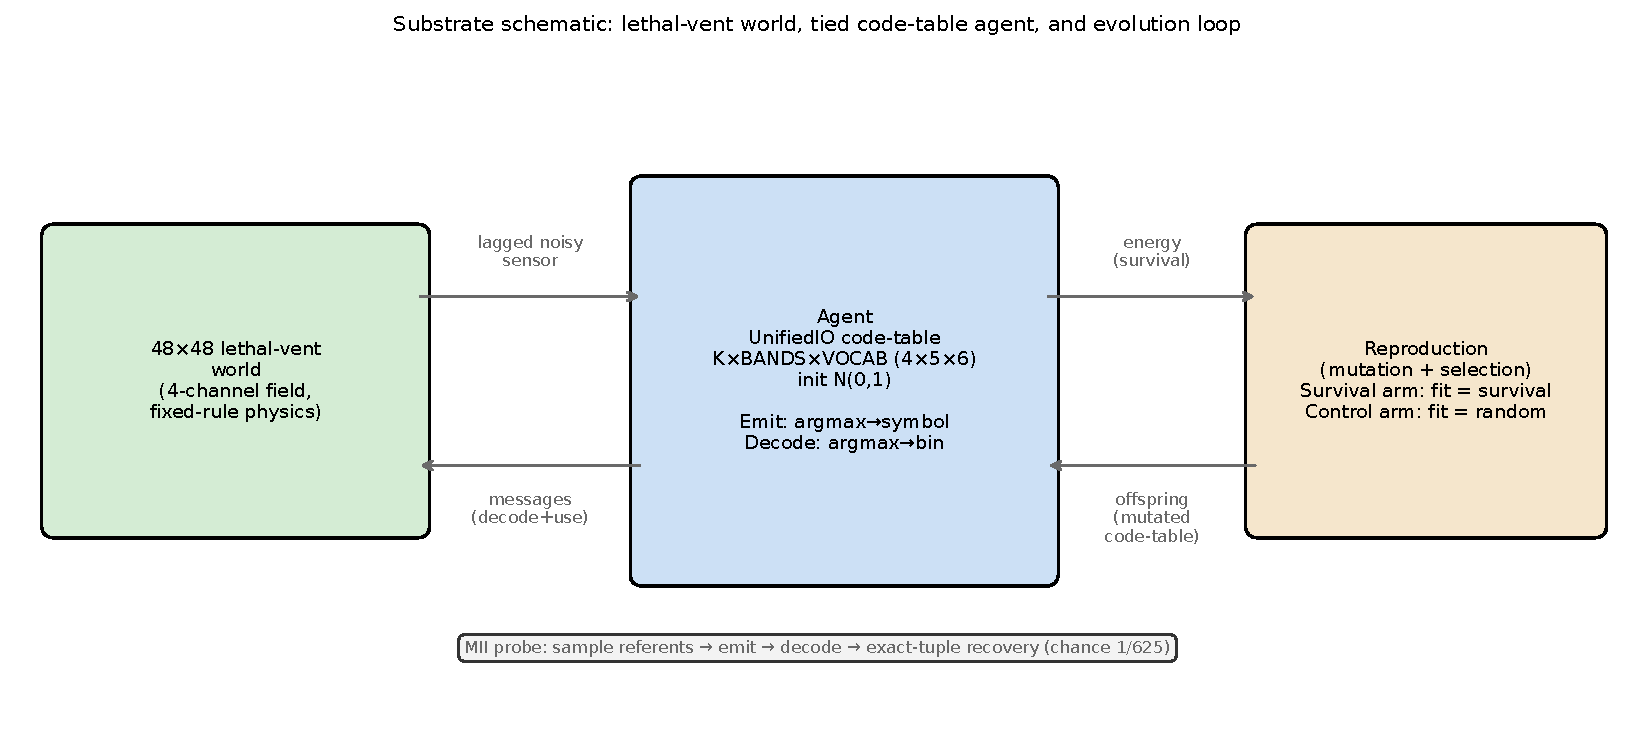
\includegraphics[width=\columnwidth]{figs/f_schematic.pdf}
  \caption{Substrate schematic: 48$\times$48 lethal-vent world, the tied \texttt{UnifiedIO}
  code-table agent ($4\times5\times6$, $\mathcal{N}(0,1)$ init), and the
  mutation-plus-selection reproduction loop. MII is measured by sampling referents, routing
  through \texttt{emit}$\to$\texttt{decode}, and scoring exact-tuple recovery
  (chance $1/625$).}
  \label{fig:schematic}
\end{figure}

This paper makes one coupled claim with two faces. \textbf{Scientifically}, in a minimal
hand-coded 2-D survival world, with no gradient on the task, no oracle or truth labels, and
no borrowed or pretrained weights, a \emph{decodable} communication channel \textbf{co-evolves
from random weights under survival selection alone}, but the result decomposes. The
architecture-matched \textbf{random-fitness control} already reaches MII \textbf{0.1174}
(\textasciitilde{}73$\times$ the 1/625 chance floor) from clonal descent alone; at the
pre-registered gen-28 fixation point survival selection then \textbf{sharpens} this channel
by a paired MII win-margin of \textbf{+0.0548 (95\% CI [0.0234, 0.0849], $n{=}48$)} (see
\Cref{fig:schematic}), a margin a secondary post-hoc probe ($n{=}24$) shows is a
\textbf{transient acceleration} that decays to a CI including zero by \textasciitilde{}gen
100. The co-evolved code remains a \textbf{private kin code}: the survival arm fixates to a
single founder lineage (dominant-lineage share 99.1\%, N$_{\rm eff}$ 1.02), within-founder
mutual intelligibility reaches $\approx 0.16$ ($\approx 100\times$ chance) while
cross-founder intelligibility sits at chance. When diversity is actively sustained (niching
at pop=96, soft96, N$_{\rm eff}$ 4.10 over 20+ generations), cross-founder intelligibility
still does not leave the floor. Across \textbf{three heterogeneous interventions} (C2X,
C2X2, C2X3) that triangulate cross-lineage pressure, cross-founder intelligibility
\emph{never rose above chance}; where the pressure bit, it only crashed survival harder. We
scope every part of this to \emph{this world and this architecture}, and to each stage's
timescale. Under these regimes a public code \emph{did not} bootstrap; we explicitly
\emph{decline to bank this as a formal negative} ($n{=}8$ positive-or-inconclusive tier).

\textbf{Methodologically}, this arc is more believable because of the bidirectional
self-audit that produced it. Its single claim is \textbf{bidirectionality} (catching
deflation as well as inflation), anchored on two in-scope, reproducible catches: a
pilot/formal false \emph{negative} (\S\ref{sec:results_coevolution}) and an RNG-offset bug
in the headline random-fitness control surfaced by a multi-model adversarial review
(\S\ref{sec:method_demo}), whose fix slightly \emph{strengthened} the margin
(+0.045 $\to$ +0.0548).

\textbf{Future work.} The arc is self-contained; it \emph{motivates rather than requires}
its sequel. The central next question is sharp: \textbf{is the public-code bottleneck the
world/ecology, or the optimizer?} We name two candidate interventions, both required to be
oracle-clean and not gradient-on-survival: (a) a richer world with spatial demes and a
resource ecology that naturally sustains coexisting lineages and provides a real survival
payoff for decoding non-kin; (b) consequence-driven lifetime learning in which agents learn
from their \emph{own} survival outcome, never supervised on the true referent. Neural
iterated learning is an established from-scratch route to structure under an imposed
transmission bottleneck \citep{ren2020}; the open problem here is doing that under survival
selection in a grounded world, without borrowing a pre-trained language or leaking the true
referent.

%% ─────────────────────────────────────────────────────────────────────────────
\appendix
\section{Reproducibility}

Every result is pinned to a durable \textbf{provenance triple}: (i) the immutable verdict
JSON frozen in git at a named commit, holding the numbers; (ii) the claim ledger
(\texttt{offscreen/CLAIM\_LEDGER.md}), indexing each claim to its verdict @ commit; and
(iii) the runbook (\texttt{offscreen/RUNBOOK.md}), giving the exact command, env vars, and
effective config per stage.

\subsection*{Run commands per stage}

All commands are issued from the repository root. \texttt{RTC\_G1F\_FORMAL=1} selects the
formal configuration; \texttt{RTC\_G1F\_FORMAL=0} is a fast pilot used only for smoke
testing. The lethal-world constant \texttt{RTC\_TOXIC\_DEATH=-0.9} is set automatically by
every g1f harness via \texttt{os.environ.setdefault}; all banked g1f-arc runs use
\texttt{-0.9}.

\begin{itemize}
\item \textbf{g1f (survival-selected channel; 28 generations):} predates the
  provenance-block discipline; reproduce as a documented multi-step sequence. (1) Run the
  $n{=}48$ RNG-fixed random-fitness control. This rngfix verdict is the \textbf{sole source}
  for every headline number. (2) The legacy helpers predate the RNG-fix and are
  \textbf{superseded}. (3) Lineage composition:
  \texttt{rtc\_g1f\_lineage\_share\_verdict.json}: dominant-share 99.1\%, N$_{\rm eff}$ 1.02.

\item \textbf{g1f transient probe (secondary, post-hoc; gen 28/56/100/150, $n{=}24$):}
  \texttt{rtc\_g1f\_transient\_probe\_verdict.json} @ddc2822.

\item \textbf{Kin-only diagnostic (28 generations):}
  \texttt{rtc\_g1f\_kinonly\_\allowbreak diagnostic\_verdict.json} @6aaefe2.

\item \textbf{C1 collapse probe (2$\times$2, 28 generations):}
  \texttt{rtc\_g1f\_c1\_collapse\_probe\_verdict.json} @21dc0f3.

\item \textbf{C2X (forced 100\% non-kin; 40 generations):}
  \texttt{rtc\_g1f\_c2x\_crosslineage\_verdict.json} @1c1a27d.

\item \textbf{C2X2 (ramped + stationary scaffold; 48 generations):}
  \texttt{rtc\_g1f\_c2x2\_ramped\_verdict.json} @07624b4.

\item \textbf{C2X3 (forced-diversity quota + 0.5 non-kin, 48 generations):}
  \texttt{rtc\_g1f\_c2x3\_forced\_verdict.json} @c9c749e.
\end{itemize}

\subsection*{CI invariants}

Heavy runs cannot be CI-automated (GPU/CPU minutes-to-hours); they are version-controlled
\emph{recipes}, not pipeline steps. What \emph{is} automated are the scale-independent
harness invariants under \texttt{tests/}, enforced on every push by
\texttt{.github/workflows/ci.yml} via \texttt{python -m pytest tests/ -q}. These guard
against silent behavior drift: vectorized MII is byte-identical to the reference loop;
\texttt{make\_provenance} produces a well-formed record; all RTC modules import cleanly; and
the no-oracle redline scan (\texttt{\_redline\_scan} over
\texttt{rtc\_g1f\_coevolve.py}) returns zero hits.

\FloatBarrier

\footnotesize
\section*{Declarations}

\textbf{Competing interests.} The author declares no competing interests.

\textbf{Funding.} This research received no specific grant from any funding agency in the public, commercial, or not-for-profit sectors.

\textbf{Use of AI tools.} AI-based tools were used to assist with drafting and language editing of this manuscript. All scientific claims, data, analyses, and conclusions are the author's own; the author verified them and takes full responsibility for the content.

\begin{thebibliography}{20}
\setlength{\itemsep}{0pt}

\bibitem[Cangelosi and Parisi(2002)]{cangelosi2002}
Cangelosi, A., \& Parisi, D. (Eds.). (2002).
\emph{Simulating the Evolution of Language}.
London: Springer-Verlag.
\url{https://doi.org/10.1007/978-1-4471-0663-0}

\bibitem[Chaabouni et~al.(2020)]{chaabouni2020}
Chaabouni, R., Kharitonov, E., Bouchacourt, D., Dupoux, E., \& Baroni, M. (2020).
Compositionality and generalization in emergent languages.
\emph{Proceedings of the 58th Annual Meeting of the Association for Computational Linguistics},
4427--4442.
\url{https://doi.org/10.18653/v1/2020.acl-main.407}

\bibitem[Flint Ashery et~al.(2025)]{ashery2025}
Flint Ashery, A., Aiello, L.~M., \& Baronchelli, A. (2025).
Emergent social conventions and collective bias in LLM populations.
\emph{Science Advances}, \textbf{11}(20), eadu9368.
\url{https://doi.org/10.1126/sciadv.adu9368}

\bibitem[Foerster et~al.(2016)]{foerster2016}
Foerster, J.~N., Assael, Y.~M., de~Freitas, N., \& Whiteson, S. (2016).
Learning to communicate with deep multi-agent reinforcement learning.
\emph{Advances in Neural Information Processing Systems 29 (NeurIPS 2016)},
2137--2145.

\bibitem[Hamilton(1964)]{hamilton1964}
Hamilton, W.~D. (1964).
The genetical evolution of social behaviour, I \& II.
\emph{Journal of Theoretical Biology}, \textbf{7}(1), 1--52.

\bibitem[Kharitonov et~al.(2019)]{kharitonov2019}
Kharitonov, E., Chaabouni, R., Bouchacourt, D., \& Baroni, M. (2019).
EGG: a toolkit for research on Emergence of lanGuage in Games.
\emph{EMNLP-IJCNLP 2019 System Demonstrations}, 55--60.
\url{https://doi.org/10.18653/v1/D19-3010}

\bibitem[Kirby et~al.(2008)]{kirby2008}
Kirby, S., Cornish, H., \& Smith, K. (2008).
Cumulative cultural evolution in the laboratory: An experimental approach to
the origins of structure in human language.
\emph{Proceedings of the National Academy of Sciences},
\textbf{105}(31), 10681--10686.
\url{https://doi.org/10.1073/pnas.0707835105}

\bibitem[Kottur et~al.(2017)]{kottur2017}
Kottur, S., Moura, J.~M.~F., Lee, S., \& Batra, D. (2017).
Natural language does not emerge `naturally' in multi-agent dialog.
\emph{EMNLP 2017}.

\bibitem[Lazaridou et~al.(2017)]{lazaridou2017}
Lazaridou, A., Peysakhovich, A., \& Baroni, M. (2017).
Multi-agent cooperation and the emergence of (natural) language.
\emph{International Conference on Learning Representations (ICLR 2017)}.
arXiv:1612.07182.

\bibitem[Lazaridou and Baroni(2020)]{lazaridoubaroni2020}
Lazaridou, A., \& Baroni, M. (2020).
Emergent multi-agent communication in the deep learning era.
arXiv:2006.02419.

\bibitem[Lewis(1969)]{lewis1969}
Lewis, D.~K. (1969).
\emph{Convention: A Philosophical Study}.
Cambridge, MA: Harvard University Press.

\bibitem[Marocco and Nolfi(2007)]{marocco2007}
Marocco, D., \& Nolfi, S. (2007).
Emergence of communication in embodied agents evolved for the ability to solve
a collective navigation problem.
\emph{Connection Science}, \textbf{19}(1), 53--74.
\url{https://doi.org/10.1080/09540090601015067}

\bibitem[Mordatch and Abbeel(2018)]{mordatch2018}
Mordatch, I., \& Abbeel, P. (2018).
Emergence of grounded compositional language in multi-agent populations.
\emph{Proceedings of the AAAI Conference on Artificial Intelligence}, \textbf{32}(1).
\url{https://doi.org/10.1609/aaai.v32i1.11492}

\bibitem[Quinn(2001)]{quinn2001}
Quinn, M. (2001).
Evolving communication without dedicated communication channels.
\emph{Advances in Artificial Life (ECAL 2001)}, LNCS 2159, pp.~357--366. Springer.
\url{https://doi.org/10.1007/3-540-44811-X_38}

\bibitem[Ren et~al.(2020)]{ren2020}
Ren, Y., Guo, S., Labeau, M., Cohen, S.~B., \& Kirby, S. (2020).
Compositional languages emerge in a neural iterated learning model.
\emph{International Conference on Learning Representations (ICLR 2020)}.

\bibitem[Skyrms(2010)]{skyrms2010}
Skyrms, B. (2010).
\emph{Signals: Evolution, Learning, and Information}.
New York: Oxford University Press.

\bibitem[Steels(2003)]{steels2003}
Steels, L. (2003).
Evolving grounded communication for robots.
\emph{Trends in Cognitive Sciences}, \textbf{7}(7), 308--312.
\url{https://doi.org/10.1016/S1364-6613(03)00129-3}

\end{thebibliography}

\end{document}
